\chapter{How a Gardener May Get Rid of the Dormice that Eat His Peaches}

Not on the same night as he had stated, but the next morning, the Count
of Monte Cristo went out by the Barrière d’Enfer, taking the road to
Orléans. Leaving the village of Linas, without stopping at the
telegraph, which flourished its great bony arms as he passed, the count
reached the tower of Montlhéry, situated, as everyone knows, upon the
highest point of the plain of that name. At the foot of the hill the
count dismounted and began to ascend by a little winding path, about
eighteen inches wide; when he reached the summit he found himself
stopped by a hedge, upon which green fruit had succeeded to red and
white flowers.

Monte Cristo looked for the entrance to the enclosure, and was not long
in finding a little wooden gate, working on willow hinges, and fastened
with a nail and string. The count soon mastered the mechanism, the gate
opened, and he then found himself in a little garden, about twenty feet
long by twelve wide, bounded on one side by part of the hedge, which
contained the ingenious contrivance we have called a gate, and on the
other by the old tower, covered with ivy and studded with wall-flowers.

No one would have thought in looking at this old, weather-beaten,
floral-decked tower (which might be likened to an elderly dame dressed
up to receive her grandchildren at a birthday feast) that it would have
been capable of telling strange things, if,—in addition to the menacing
ears which the proverb says all walls are provided with,—it had also a
voice.

The garden was crossed by a path of red gravel, edged by a border of
thick box, of many years’ growth, and of a tone and color that would
have delighted the heart of Delacroix, our modern Rubens. This path was
formed in the shape of the figure of 8, thus, in its windings, making a
walk of sixty feet in a garden of only twenty.

Never had Flora, the fresh and smiling goddess of gardeners, been
honored with a purer or more scrupulous worship than that which was
paid to her in this little enclosure. In fact, of the twenty rose-trees
which formed the \textit{parterre}, not one bore the mark of the slug, nor
were there evidences anywhere of the clustering aphis which is so
destructive to plants growing in a damp soil. And yet it was not
because the damp had been excluded from the garden; the earth, black as
soot, the thick foliage of the trees betrayed its presence; besides,
had natural humidity been wanting, it could have been immediately
supplied by artificial means, thanks to a tank of water, sunk in one of
the corners of the garden, and upon which were stationed a frog and a
toad, who, from antipathy, no doubt, always remained on the two
opposite sides of the basin. There was not a blade of grass to be seen
in the paths, or a weed in the flower-beds; no fine lady ever trained
and watered her geraniums, her cacti, and her rhododendrons, in her
porcelain \textit{jardinière} with more pains than this hitherto unseen
gardener bestowed upon his little enclosure.

Monte Cristo stopped after having closed the gate and fastened the
string to the nail, and cast a look around.

“The man at the telegraph,” said he, “must either engage a gardener or
devote himself passionately to agriculture.”

Suddenly he struck against something crouching behind a wheelbarrow
filled with leaves; the something rose, uttering an exclamation of
astonishment, and Monte Cristo found himself facing a man about fifty
years old, who was plucking strawberries, which he was placing upon
grape leaves. He had twelve leaves and about as many strawberries,
which, on rising suddenly, he let fall from his hand.

“You are gathering your crop, sir?” said Monte Cristo, smiling.

\begin{figure}[ht]
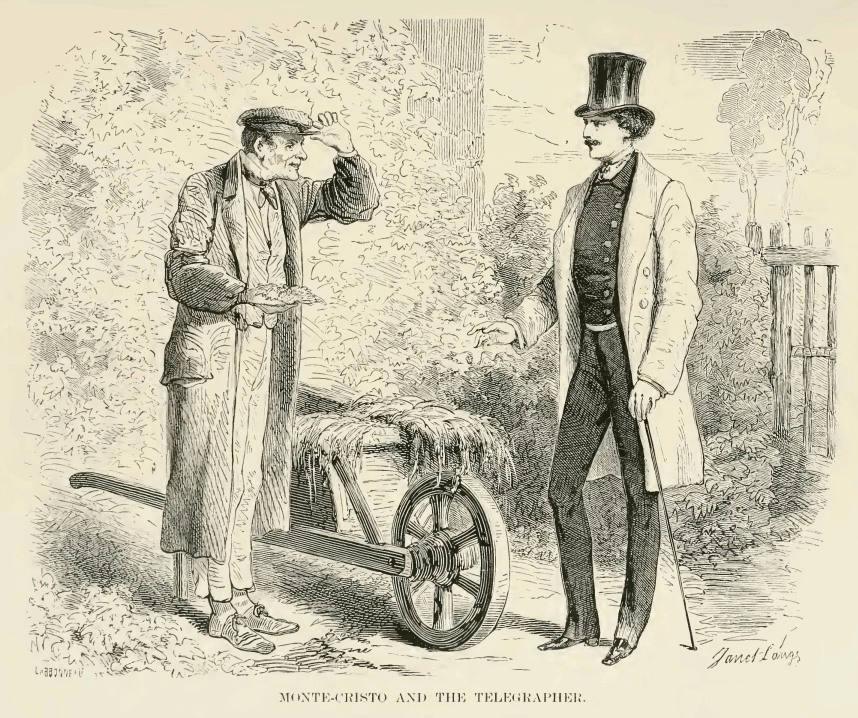
\includegraphics[width=\textwidth]{30193m.jpg}
\end{figure}

“Excuse me, sir,” replied the man, raising his hand to his cap; “I am
not up there, I know, but I have only just come down.”

“Do not let me interfere with you in anything, my friend,” said the
count; “gather your strawberries, if, indeed, there are any left.”

“I have ten left,” said the man, “for here are eleven, and I had
twenty-one, five more than last year. But I am not surprised; the
spring has been warm this year, and strawberries require heat, sir.
This is the reason that, instead of the sixteen I had last year, I have
this year, you see, eleven, already plucked—twelve, thirteen, fourteen,
fifteen, sixteen, seventeen, eighteen. Ah, I miss three, they were here
last night, sir—I am sure they were here—I counted them. It must be the
son of Mère Simon who has stolen them; I saw him strolling about here
this morning. Ah, the young rascal—stealing in a garden—he does not
know where that may lead him to.”

“Certainly, it is wrong,” said Monte Cristo, “but you should take into
consideration the youth and greediness of the delinquent.”

“Of course,” said the gardener, “but that does not make it the less
unpleasant. But, sir, once more I beg pardon; perhaps you are an
officer that I am detaining here.” And he glanced timidly at the
count’s blue coat.

\begin{figure}[ht]
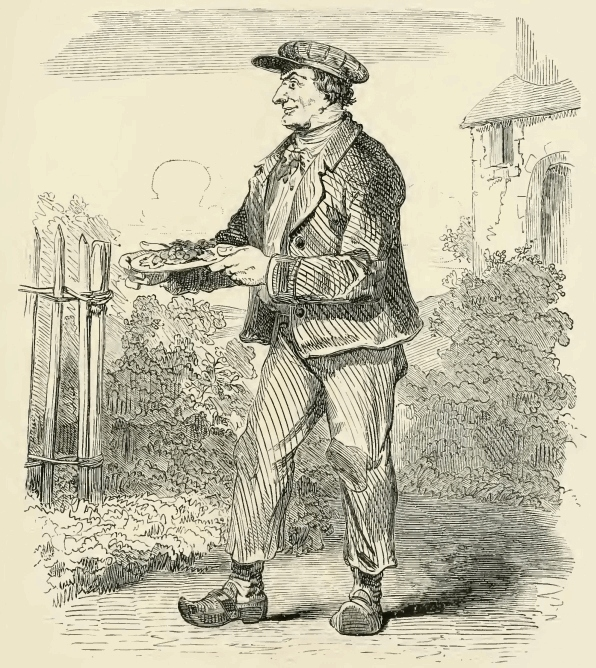
\includegraphics[width=\textwidth]{30197m.jpg}
\end{figure}

“Calm yourself, my friend,” said the count, with the smile which he
made at will either terrible or benevolent, and which now expressed
only the kindliest feeling; “I am not an inspector, but a traveller,
brought here by a curiosity he half repents of, since he causes you to
lose your time.”

“Ah, my time is not valuable,” replied the man with a melancholy smile.
“Still it belongs to government, and I ought not to waste it; but,
having received the signal that I might rest for an hour” (here he
glanced at the sun-dial, for there was everything in the enclosure of
Montlhéry, even a sun-dial), “and having ten minutes before me, and my
strawberries being ripe, when a day longer—by-the-by, sir, do you think
dormice eat them?”

“Indeed, I should think not,” replied Monte Cristo; “dormice are bad
neighbors for us who do not eat them preserved, as the Romans did.”

“What? Did the Romans eat them?” said the gardener—“ate dormice?”

“I have read so in Petronius,” said the count.

“Really? They can’t be nice, though they do say ‘as fat as a dormouse.’
It is not a wonder they are fat, sleeping all day, and only waking to
eat all night. Listen. Last year I had four apricots—they stole one, I
had one nectarine, only one—well, sir, they ate half of it on the wall;
a splendid nectarine—I never ate a better.”

“You ate it?”

“That is to say, the half that was left—you understand; it was
exquisite, sir. Ah, those gentlemen never choose the worst morsels;
like Mère Simon’s son, who has not chosen the worst strawberries. But
this year,” continued the horticulturist, “I’ll take care it shall not
happen, even if I should be forced to sit by the whole night to watch
when the strawberries are ripe.”

Monte Cristo had seen enough. Every man has a devouring passion in his
heart, as every fruit has its worm; that of the telegraph man was
horticulture. He began gathering the grape-leaves which screened the
sun from the grapes, and won the heart of the gardener.

“Did you come here, sir, to see the telegraph?” he said.

“Yes, if it isn’t contrary to the rules.”

“Oh, no,” said the gardener; “not in the least, since there is no
danger that anyone can possibly understand what we are saying.”

“I have been told,” said the count, “that you do not always yourselves
understand the signals you repeat.”

“That is true, sir, and that is what I like best,” said the man,
smiling.

“Why do you like that best?”

“Because then I have no responsibility. I am a machine then, and
nothing else, and so long as I work, nothing more is required of me.”

“Is it possible,” said Monte Cristo to himself, “that I can have met
with a man that has no ambition? That would spoil my plans.”

“Sir,” said the gardener, glancing at the sun-dial, “the ten minutes
are almost up; I must return to my post. Will you go up with me?”

“I follow you.”

Monte Cristo entered the tower, which was divided into three stories.
The tower contained implements, such as spades, rakes, watering-pots,
hung against the wall; this was all the furniture. The second was the
man’s conventional abode, or rather sleeping-place; it contained a few
poor articles of household furniture—a bed, a table, two chairs, a
stone pitcher—and some dry herbs, hung up to the ceiling, which the
count recognized as sweet peas, and of which the good man was
preserving the seeds; he had labelled them with as much care as if he
had been master botanist in the Jardin des Plantes.

“Does it require much study to learn the art of telegraphing?” asked
Monte Cristo.

“The study does not take long; it was acting as a supernumerary that
was so tedious.”

“And what is the pay?”

“A thousand francs, sir.”

“It is nothing.”

“No; but then we are lodged, as you perceive.”

Monte Cristo looked at the room. They passed to the third story; it was
the telegraph room. Monte Cristo looked in turn at the two iron handles
by which the machine was worked. “It is very interesting,” he said,
“but it must be very tedious for a lifetime.”

“Yes. At first my neck was cramped with looking at it, but at the end
of a year I became used to it; and then we have our hours of
recreation, and our holidays.”

“Holidays?”

“Yes.”

“When?”

“When we have a fog.”

“Ah, to be sure.”

“Those are indeed holidays to me; I go into the garden, I plant, I
prune, I trim, I kill the insects all day long.”

“How long have you been here?”

“Ten years, and five as a supernumerary make fifteen.”

“You are——”

“Fifty-five years old.”

“How long must you have served to claim the pension?”

“Oh, sir, twenty-five years.”

“And how much is the pension?”

“A hundred crowns.”

“Poor humanity!” murmured Monte Cristo.

“What did you say, sir?” asked the man.

“I was saying it was very interesting.”

“What was?”

“All you were showing me. And you really understand none of these
signals?”

“None at all.”

“And have you never tried to understand them?”

“Never. Why should I?”

“But still there are some signals only addressed to you.”

“Certainly.”

“And do you understand them?”

“They are always the same.”

“And they mean——”

“‘\textit{Nothing new; You have an hour;}’ or ‘\textit{Tomorrow}.’”

“This is simple enough,” said the count; “but look, is not your
correspondent putting itself in motion?”

“Ah, yes; thank you, sir.”

“And what is it saying—anything you understand?”

“Yes; it asks if I am ready.”

“And you reply?”

“By the same sign, which, at the same time, tells my right-hand
correspondent that I am ready, while it gives notice to my left-hand
correspondent to prepare in his turn.”

“It is very ingenious,” said the count.

“You will see,” said the man proudly; “in five minutes he will speak.”

“I have, then, five minutes,” said Monte Cristo to himself; “it is more
time than I require. My dear sir, will you allow me to ask you a
question?”

“What is it, sir?”

“You are fond of gardening?”

“Passionately.”

“And you would be pleased to have, instead of this terrace of twenty
feet, an enclosure of two acres?”

“Sir, I should make a terrestrial paradise of it.”

“You live badly on your thousand francs?”

“Badly enough; but yet I do live.”

“Yes; but you have a wretchedly small garden.”

“True, the garden is not large.”

“And, then, such as it is, it is filled with dormice, who eat
everything.”

“Ah, they are my scourges.”

“Tell me, should you have the misfortune to turn your head while your
right-hand correspondent was telegraphing——”

“I should not see him.”

“Then what would happen?”

“I could not repeat the signals.”

“And then?”

“Not having repeated them, through negligence, I should be fined.”

“How much?”

“A hundred francs.”

“The tenth of your income—that would be fine work.”

“Ah!” said the man.

“Has it ever happened to you?” said Monte Cristo.

“Once, sir, when I was grafting a rose-tree.”

“Well, suppose you were to alter a signal, and substitute another?”

“Ah, that is another case; I should be turned off, and lose my
pension.”

“Three hundred francs?”

“A hundred crowns, yes, sir; so you see that I am not likely to do any
of these things.”

“Not even for fifteen years’ wages? Come, it is worth thinking about?”

“For fifteen thousand francs?”

“Yes.”

“Sir, you alarm me.”

“Nonsense.”

“Sir, you are tempting me?”

“Just so; fifteen thousand francs, do you understand?”

“Sir, let me see my right-hand correspondent.”

“On the contrary, do not look at him, but at this.”

“What is it?”

“What? Do you not know these bits of paper?”

“Bank-notes!”

“Exactly; there are fifteen of them.”

“And whose are they?”

“Yours, if you like.”

“Mine?” exclaimed the man, half-suffocated.

“Yes; yours—your own property.”

“Sir, my right-hand correspondent is signalling.”

“Let him signal.”

“Sir, you have distracted me; I shall be fined.”

“That will cost you a hundred francs; you see it is your interest to
take my bank-notes.”

“Sir, my right-hand correspondent redoubles his signals; he is
impatient.”

“Never mind—take these;” and the count placed the packet in the man’s
hands. “Now this is not all,” he said; “you cannot live upon your
fifteen thousand francs.”

“I shall still have my place.”

“No, you will lose it, for you are going to alter your correspondent’s
message.”

“Oh, sir, what are you proposing?”

“A jest.”

“Sir, unless you force me——”

“I think I can effectually force you;” and Monte Cristo drew another
packet from his pocket. “Here are ten thousand more francs,” he said,
“with the fifteen thousand already in your pocket, they will make
twenty-five thousand. With five thousand you can buy a pretty little
house with two acres of land; the remaining twenty thousand will bring
you in a thousand francs a year.”

“A garden with two acres of land!”

“And a thousand francs a year.”

“Oh, heavens!”

“Come, take them,” and Monte Cristo forced the bank-notes into his
hand.

“What am I to do?”

“Nothing very difficult.”

“But what is it?”

“To repeat these signs.” Monte Cristo took a paper from his pocket,
upon which were drawn three signs, with numbers to indicate the order
in which they were to be worked.

“There, you see it will not take long.”

“Yes; but——”

“Do this, and you will have nectarines and all the rest.”

The shot told; red with fever, while the large drops fell from his
brow, the man executed, one after the other, the three signs given by
the count, in spite of the frightful contortions of the right-hand
correspondent, who, not understanding the change, began to think the
gardener had gone mad. As to the left-hand one, he conscientiously
repeated the same signals, which were finally transmitted to the
Minister of the Interior.

“Now you are rich,” said Monte Cristo.

“Yes,” replied the man, “but at what a price!”

“Listen, friend,” said Monte Cristo. “I do not wish to cause you any
remorse; believe me, then, when I swear to you that you have wronged no
man, but on the contrary have benefited mankind.”

The man looked at the bank-notes, felt them, counted them, turned pale,
then red, then rushed into his room to drink a glass of water, but he
had no time to reach the water-jug, and fainted in the midst of his
dried herbs. Five minutes after the new telegram reached the minister,
Debray had the horses put to his carriage, and drove to Danglars’
house.

“Has your husband any Spanish bonds?” he asked of the baroness.

“I think so, indeed! He has six millions’ worth.”

“He must sell them at whatever price.”

“Why?”

“Because Don Carlos has fled from Bourges, and has returned to Spain.”

\begin{figure}[ht]
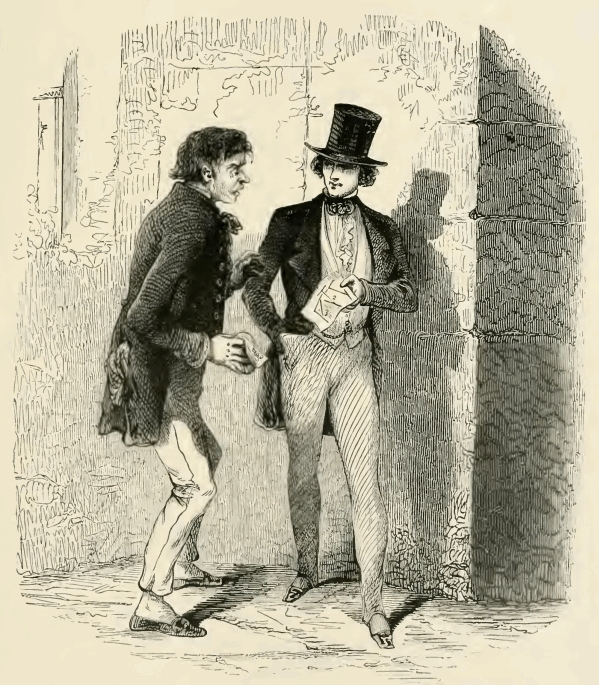
\includegraphics[width=\textwidth]{30203m.jpg}
\end{figure}

“How do you know?” Debray shrugged his shoulders.

“The idea of asking how I hear the news,” he said.

The baroness did not wait for a repetition; she ran to her husband, who
immediately hastened to his agent, and ordered him to sell at any
price. When it was seen that Danglars sold, the Spanish funds fell
directly. Danglars lost five hundred thousand francs; but he rid
himself of all his Spanish shares. The same evening the following was
read in \textit{Le Messager}:

“[By telegraph.] The king, Don Carlos, has escaped the vigilance of his
guardians at Bourges, and has returned to Spain by the Catalonian
frontier. Barcelona has risen in his favor.”

All that evening nothing was spoken of but the foresight of Danglars,
who had sold his shares, and of the luck of the stock-jobber, who only
lost five hundred thousand francs by such a blow. Those who had kept
their shares, or bought those of Danglars, looked upon themselves as
ruined, and passed a very bad night. Next morning \textit{Le Moniteur}
contained the following:

“It was without any foundation that \textit{Le Messager} yesterday announced
the flight of Don Carlos and the revolt of Barcelona. The king (Don
Carlos) has not left Bourges, and the peninsula is in the enjoyment of
profound peace. A telegraphic signal, improperly interpreted, owing to
the fog, was the cause of this error.”

The funds rose one per cent higher than before they had fallen. This,
reckoning his loss, and what he had missed gaining, made the difference
of a million to Danglars.

“Good,” said Monte Cristo to Morrel, who was at his house when the news
arrived of the strange reverse of fortune of which Danglars had been
the victim, “I have just made a discovery for twenty-five thousand
francs, for which I would have paid a hundred thousand.”

“What have you discovered?” asked Morrel.

“I have just discovered how a gardener may get rid of the dormice that
eat his peaches.”
